\section{Lightweight Nondeterminism
  Detection}

\begin{figure}
  \centering
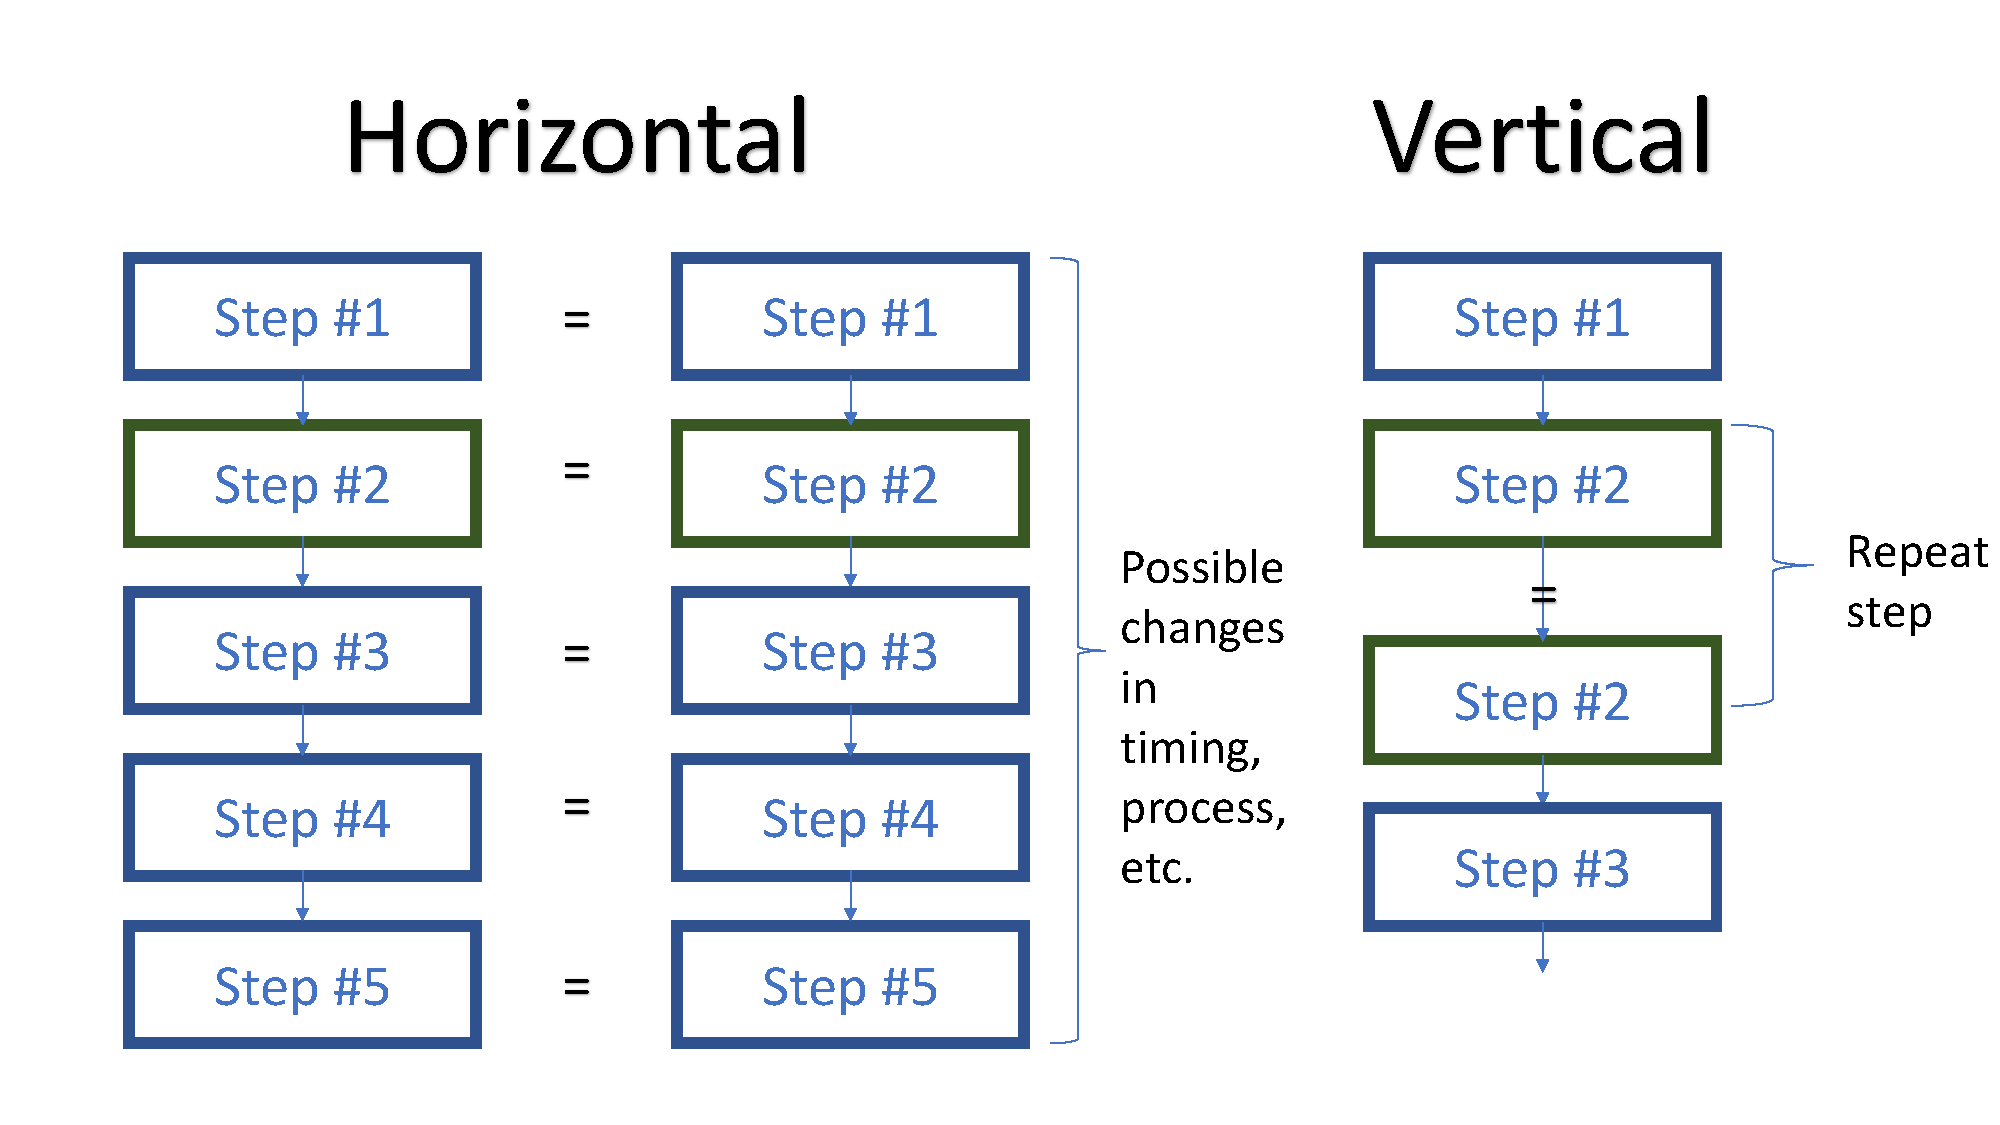
\includegraphics[width=0.6\columnwidth]{types}
\caption{Types of determinism}
\label{fig:types}
\end{figure}

We define two basic types of determinism, shown in Figure
\ref{fig:types}:  \emph{horizontal} and \emph{vertical} determinism.  In
horizontal determinism a software system reliably
produces the same behavior given the same steps of a test: the
behavior of multiple executions that are ``the same'' in terms of
inputs/actions can be aligned and checked for equality.  In
vertical determinism, rather than behavior across executions, we are
interested in behavior within an execution, where repeating the same
step of a test twice should result in the same behavior.  Vertical determinism is both rarer and more specialized than
horizontal determinism.

\subsection{Horizontal Determinism}


\subsubsection{Determinism and Reflexive Differential Testing}

Horizontal determinism can be best understood by thinking of
nondeterminism detection as an unusual kind of \emph{differential
  testing} \cite{Differential,ICSEDiff}.  In differential testing, a
system is compared against a reference in order to ensure that
it behaves equivalently, at some level of abstraction, to another
implementation.  Differential testing is
extremely powerful, in that any (properly defined) divergence of
behavior indicates a functional correctness fault in (at
least) one of the systems under test, and  is widely
used for systems software such as compilers
\cite{Differential,csmith} and file systems \cite{CFV08,AMAI}.  The major limitation of differential
testing is that multiple implementations of a system are
almost as rare as good correctness specifications.
For the special case of detecting nondeterminism, however, \emph{a
  system can serve as its own reference implementation.}    The
problem, then, becomes one of deciding at what granularity the
reference equivalence will be checked:  e.g., 
processor-instruction and memory-layout determinism is seldom
necessary or even desired.  We propose two approaches to ``aligning'' an
execution with itself.

\emph{Visible value determinism} uses the human-accessible outputs (displayed
or stored to a file), and \emph{values returned by functions or methods
called as a library by other code}, as the criteria for determining if two executions
are equivalent.  Determinism is motivated by the
desire to create consistent behavior for an observer, whether that
observer is a human user, another software system, or a regression
test.  In practice, of course, some values (time
stamps, pointer addresses, etc.) are not expected to be deterministic
by an observer; we call these values \emph{opaque} in that they are
not interpretable as ``showing'' the internal workings of the code
being tested for determinism.  Rather, they mask an abstraction,
usually one managed by the operating system (system
time, memory management).   Any mechanism for visible value
determinism needs to support designation of some
values as opaque.

While visisble value determinism provides very fine granularity, which
is important for debugging purposes, it is also expensive, requiring
checks on a potentially very large number of values.  It is often
sufficient to only compare final states of a computation performed by
the system, which we refer to as \emph{final state determinism}.


%\subsubsection{Core Sources of Difference:  Timing and Process}

\subsection{Vertical Determinism}

Vertical determinism is a property that expresses that some operations
of a software system should, within the same trace, always behave the
same way.  Usually, for interesting cases, this is dependent on some
state of the system, though some operations should be completely
state-independent.  E.g, the hash of a given bytestring returned by a
security library should never change.  This is one aspect of
\emph{pure} functions.  For nondeterminism checking, the interesting
cases are non-pure: a function depends on system state, but should
always depend on it in the same way, and should not, itself, change
system state in a way that would change its behavior on a subsequent
call to that function.

Many \emph{idempotent} operations fall into this category.
Consider adding an element to an AVL tree implementing a set, not a
multiset.  Assume the method call returns the parent node of the
element, whether it was added or was already in the tree.  Calling
this method any number of times in a row should always return the
same value.  One approach, then, would be to identify
idempotent operations 
automatically retry all such operations, checking that the
result is unchanged.  Identifying idempotent operations, however, imposes a specification burden.

%\subsubsection{Failure Determinism}

However, for the specialized case of  failure determinism, no
specification is required.
Failure determinism is the following restriction on an API: {\bf If a call/action \emph{fails}, and indicates this to the caller, it should not modify system
  state in any way; changes should be ``rolled back.''}   Some behaviors of the Mac OS High Sierra
root exploit (CVE-2017-13872 \cite{applebug0}) exhibited failure
nondeterminism.  Attempting to login with the root account with an
empty password appeared to fail, then, on a repeated try, succeeded
\cite{applebug1,applebug2}.   Many library APIs are largely failure deterministic.  For instance, if
we exclude actual I/O errors, most POSIX file system calls either
succeed or do nothing; interfaces that may only partially succeed,
such as {\tt read} and {\tt write} tend to explicitly return a degree of success, rather than signalling total failure, when appropriate.  

In languages with a clear mechanism for expressing failure of a call
(e.g., exceptions in Python and Java, or Option/Result types in Rust,
Haskell, and ML), failure determinism can be automatically checked.
The overhead should be even lower than for other vertical determinism, in that we can expect most failing
operations to be fast.  Checking equivalence of full
observable state, however, is still expensive, and requires defining
the observable components of a state.  A more lightweight, but (as we
will show) still powerful way of checking for failure nondeteterminism
is to simply
\emph{repeat the failing operation, and check if it still fails}.  This more restrictive notion still captures such issues as the Apple login bug. 

\begin{comment}
\subsection{Nondeterminism vs. Flakiness}

A key concept in this paper is that flaky tests (tests that sometimes
pass and sometimes fail, recall) exist due to underlying
nondeterministic behavior.  Our interest is in identifying such
nondeterministic behavior, not in addressing flakiness \emph{per se}.
Of course, the concepts are closely related.  We make ``did not behave
nondeterministically'' an additional \emph{property} that a test can
fail.  Due to the nature of (horizontal) nondeterminism, such failure
is almost always going to be inherently flaky---sometimes a test
will behave nondeterministically, and sometimes it will not.  But the
idea is a separate one from flakiness; in order to show horizontal
nondeterminism, we need only see a change in values in a test, not in
the disposition (failed/passed) of the test.
%\begin{comment}
  It may be that, without
the additional property of determinism, the change cannot actually
cause failure, and thus flakiness.  The real relationship between our
nondeterminism and flakiness is that tests (automatically generated or
manually constructued) that rely on code that can be shown to exhibit
horizontal nondeterminism contain a potential source of flakiness.  If
the code behaves nondeterministically, and the values that are
observed to change can flow to influence the outcome of the test,
flakiness may well result.
%\end{comment}
Vertical nondeterminism, in fact, is usually \emph{completely} unrelated
to flakiness, in that some bugs (improper handling of hardware errors
in a file system, for example) produce \emph{reliably}
``nondeterministic'' (from a software library users' point of view)
behavior. The behavior is only
``nondeterministic'' from a caller's point of view in that
there is an expectation that a call will always ``do the same thing,
under the same circumstances'' which is the \emph{conceptual} common
factor in ``determinism.''
\end{comment}

\subsection{Formal Definitions}
\label{sec:formal}

We can formally distinguish the types of nondeterminism by using a
variant of a labeled transition system (LTS), where (1) $S$
is a set of states; (2) $V$ is a set of \emph{observable} states, where
$|V| \leq |S|$; (3) $v: S \rightarrow V$ is a total function that, given a state, maps it
  into the set of observable states, such that every state has an observable
  component, which may be the complete state, or only an aspect of the
  full state; (4)  $I \subseteq S$ is a set of initial states; (5) $A$
  is a set of \emph{actions}; and (6) $T \subseteq S \times A \times S$ is a transition relation.

  \begin{comment}
\begin{itemize}
\item $S$ is a set of states.
\item $V$ is a set of \emph{observable} states, where $|V| \leq |S|$.
\item $v: S \rightarrow V$ is a total function that, given a state, maps it
  into the set of observable states.  Every state has an observable
  component, which may be the complete state, or only an aspect of the
  full state; we even allow $V$ to contain a
  single element, in which case no two states in $S$ can be
  distinguished by an observer.
\item $I \subseteq S$ is a set of initial states.
\item $A$ is a set of \emph{actions}.
\item $T \subseteq S \times A \times S$ is a transition relation.
\end{itemize}
\end{comment}

We assume that the \emph{underlying} behavior of a system may be
deterministic, or nondeterministic  by allowing
for a transition relation that \emph{may} be a function of
$S \times A$.  A \emph{trace} $t$ is a finite sequence $t = s_0
\xrightarrow[]{\alpha_0} s_1 \xrightarrow[]{\alpha_1} \ldots
\xrightarrow[]{\alpha_{n-1}} s_n$ where $s_0 \in I$ and $\forall i < n
. (s_i, \alpha_i, s_{i+1}) \in T$.  The concept of an action does not restrict this approach to reactive
systems; it can be generalized to consider the only action that varies
to be the selection of an input, $\alpha_0$, with the remainder of the
actions being internal $\tau$ actions.

\subsubsection{Horizontal Determinism}

A pair of traces $(t_1, t_2)$ where $t_1 = s^1_0
\xrightarrow[]{\alpha^1_0} s^1_1 \xrightarrow[]{\alpha^1_1} \ldots
\xrightarrow[]{\alpha^1_{n-1}} s^1_n$ and $t_2 = s^2_0
\xrightarrow[]{\alpha^2_0} s_1 \xrightarrow[]{\alpha^2_1} \ldots
\xrightarrow[]{\alpha^2_{n-1}} s^2_n$ are said to show \emph{visible value
  nondeterminism} if $\exists i > 0$ such that: $\forall j < i . \alpha^1_j = \alpha^2_j \wedge
v(s^1_j) = v(s^2_j)$ but $v(s^1_i) \neq v(s^2_i)$.  \emph{Final state
  nondeterminism} is defined in the same way, except with the
restriction that $i = n$.  A pair of traces may exhibit visible value
nondeterminism but not final state nondeterminism.

\begin{comment}
A point to emphasize is that while horizontal determinism
requires two traces, it does not require a test generation algorithm
to \emph{produce} pairs of traces, which would require substantial
modification of most such tools (e.g., random testers or fuzzers, and
even model checkers), only to find an
action sequence or input which, when executed twice, produces a $t_1$ and $t_2$
meeting the requirements for showing nondeterminism.
\end{comment}

\begin{comment}In general, testing tools do not produce
\emph{traces}, they produce \emph{action sequences} or \emph{inputs}.  The two traces
used to show nondeterminism, by definition, have the same action
sequences, which means that a testing tool only needs to search for an
action sequence or input which, when executed twice, produces a $t_1$ and $t_2$
meeting the requirements for showing nondeterminism ---
non-equivalence of $v(s)$ for some $s$.
\end{comment}

\subsubsection{Vertical Determinism}

To define vertical nondeterminism with
respect to idempotency, we can
define $\mathcal{I} \subseteq A$, the set of \emph{idempotent}
actions.  A trace $t s_0
\xrightarrow[]{\alpha_0} s_1 \xrightarrow[]{\alpha_1} \ldots
\xrightarrow[]{\alpha_{n-1}} s_n$ shows \emph{vertical nondeterminism
  with respect to idempotent operations} if $\exists i < n$ such that
$\alpha_i \in \mathcal{I} \wedge \alpha_i = \alpha_{i+1}$ and $v(s_{i+1})
\neq v(s_{i+2})$.  Note that vertical nondeterminism may, in theory, exhibit only
after a sequence of more than two successive applications of a (supposedly)
idempotent operation; the definition only requires that after \emph{some}
sequence of actions, possibly with $\alpha_{i-1} = \alpha_i$, the
visible state changes.  In an implementation, we would usually restrict the
search to a finite number of repetitions; for many faults, two
``copies'' will suffice.
%Only the existence of \emph{non-visible} state changes that
%can eventually produce visible state changes \emph{after a succession of the
%same action} require more repetitions.

\subsubsection{Failure Determinism}

To define failure nondeterminism, we extend the
transition relation to include a notion of \emph{failure}: $T \subseteq S
\times A \times S \times {\tt F: bool}$, where the boolean $F$ indicates
whether the action $A$ \emph{failed}.   A trace $t = s_0
\xrightarrow[]{\alpha_0} (s_1, F_0) \xrightarrow[]{\alpha_1} \ldots
\xrightarrow[]{\alpha_{n-1}} (s_n, F_{n-1})$ shows \emph{failure
  nondeterminism} if $\exists i$ such that $F_{i}$ (that is,
$\alpha_i$ \emph{fails}) and either (1) $v(s_{i}) \neq v(s_{i+1})$
(the visible state changes) or (2)
$\alpha_i = \alpha_{i+1} \wedge \neg F_{i+1}$ (the same action is
repeated, but this time does not fail).  The second possibility
offers a \emph{lightweight} approach to checking for failure
nondeterminism.  Unlike all of the other ways to demonstrate
nondeterminism we consider, this second type of failure nondeterminism does not
require the use of $v$.

\subsection{Sources of Nondeterminism}
\label{sec:sources}

In order to implement a practical nondeterminism-detection tool, it is
important to consider the real-world sources of nondeterminism.  
\begin{comment}
Most of these
sources can, in principle, be detected simply by re-running a test
twice and comparing results, either at all visible values or at the
final state.  For example, if some library call uses a random number
generator (perhaps in a stochastic algorithm), the returned value should be
different on a second run.  Timing dependencies may change on a second
execution, especially if a delay is added between steps of the test (a
more principled version of the unfortunate tradition of testing
concurrent code by adding ad-hoc {\tt sleep} statements).
\end{comment}
Most nondeterministic behavior in tests is probably attributable to simple
effects that can vary with a repeated execution, in the same
(approximate) enviroment, of the same test.  There are two broad classes of
nondeterminism that can usually be detected by
executing the same test twice in succession, without attempting
to control any other factors.  {\bf External Environment} nondeterminism arises
  when a test's behavior depends on factors outside the program under
  test, which are subject to uncontrolled variance.  Calling {\tt
    random()} in Python is an obvious example. Similarly, calls to {\tt time}
  functions  will usually return different values on different runs,
  and even if only elapsed time is used, due to system load, I/O, and
  other external factors.  {\bf Concurrency} is a second common cause for
  nondeterminism, when an algorithm is implemented using
  concurrency, in the (incorrect) belief that the result of the
  algorithm remains deterministic.  E.g., a multi-threaded
  implementation of a search algorithm, that returns the location of
  an item in an unsorted list; in the presence of duplicate items,
  thread scheduling may change the index returned.  Lam et al. \cite{idflakies} note that flaky tests not due to order
dependence are generally due to ``concurrency, timeouts,
network/IO, etc.'' a description that is well accounted for by these two
primary sources.

\begin{comment}
\begin{itemize}
\item {\bf External Environment:} This class of nondeterminism arises
  when a test's behavior depends on factors outside the program under
  test, which are subject to uncontrolled variance.  Calling {\tt
    random()} in Python is an obvious example. Similarly, calls to {\tt time}
  functions  will usually return different values on different runs,
  and even if only elapsed time is used, due to system load, I/O, and
  other external factors.
  %Finally, in
  %distributed system testing, the environment is often remote servers
  %(or clients) that may be unavailable, slower than expected, or
  %subject to faulty behavior for reasons not under the control of the
  %test.
\item {\bf Concurrency:} A second common cause for
  nondeterminism in tests is when an algorithm is implemented using
  concurrency, in the (incorrect) belief that the result of the
  algorithm remains deterministic.  E.g., a multi-threaded
  implementation of a search algorithm, that returns the location of
  an item in an unsorted list; in the presence of duplicate items, thread scheduling may change the index returned.
  %If the list may contain duplicates,
  %and a developer has not accounted for this possibility, the
  %algorithm may return different locations of an item
  %depending on the scheduling of threads.
  %Arguably, this can be
  %subsumed under the first class, with the behavior of the
  %processor/scheduler as the ``enviromental'' factor; relying on
  %scheduling is, in a sense, equivalent to calling {\tt random} or
  %{\tt time}.
\end{itemize}
\end{comment}

%, and most of which can be detected easily
%, at least in principle, 
%by multiple runs of a test.
%However, simply running a test twice in the same process (possibly with a delay between steps) does
%not suffice in all cases.

\subsubsection{Process-Based Nondeterminism}

\label{sec:pnondet}

Some sources of nondeterminism unfortunately require executing a test in a \emph{new
process environment}, because the source is inherently tied to the
process in which code runs.  In terms of our formalism, an
action needs to be introduced that indicates the generation of a fresh
process.  Address Space Layout Randomization (ASLR) \cite{ASLR}  is probably the most
important source of nondeterminism that arises (only) from change in
process.  ASLR scrambles the layout of memory of the process in which
an executable runs in order to make it harder to exploit memory-safety
vulnerabilities in code, but also makes tests more flaky
%as nondeterminism.

Another example of process-based nondeterminism was discovered by numerous Python developers when Python
version 3.3 introduced automatic random salting of hashes on a
per-process basis,
in order to mitigate hash-based denial of service attacks
\cite{denial}.  Until version 3.6 this not only resulted in changes in
exact hash values, but in the order of iteration on
dictionaries; in Python 3.6, the default dictionary implementation became an ordered dictionary with consistent iteration, though actual hashes remained nondeterministic.  While few programs relied on exact hash values, many
relied on a
predictable order for dictionary iteration.  Testing
Python code for nondeterminism based on hash seed requires
running in a new process:  Python does not allow changing the salt.

%Other, less common, effects tied to process also exist.  A few tests
%may somehow depend on their actual PID (Process ID) or at least the
%parent process' ID.  Process change increases the likelihood that on a multi-core
%system a test will execute on a different CPU than in the first
%execution, which can have many subtle effects, mostly related to
%changed timing.

%One common cause of flaky tests is \emph{test order dependence} \cite{idflakies}.  This
%is less of a concern in our setting, since many problems due to test
%order are easily exposed in random testing, since the
%order-dependence-inducing operations will seldom happen in the
%same order in randomly generated tests.
%For example, consider the
%case where a test usually run ``early'' initializes an uninitialized
%value in a system, and a later test will only fail if it somehow is
%run before the initializing test.  In random testing, the order of
%initialization/access is likely to be random, and some run of a random
%tester is likely to expose the problem as a (deterministic, not flaky) failure.
%However, for cases where
%there is an order dependence that is hard to translate into an
%actual bug, using a fresh
%process may expose such dependencies---the ``environment'' of the
%parent process will have the, e.g., a flag set or value initialized, but
%the new process will not.

\section{Probabilistic Test Reduction}

Delta-debugging \cite{DD}  is a widely used method for reducing the
size of failing tests, making them easier to understand and debug.
The core idea of delta-debugging is to take a test with some
property (usually ``it fails'')
and produce a smaller test that has the same property.
Delta-debugging as originally proposed uses a
modified binary search, but we rely only on the general structure: \cite{CReduce,onetest}:  Given a
test case, $T_{\mathit{INIT}} : \mathit{test}$ and a predicate
$\mathit{PRED}: \mathit{test} \rightarrow \mathit{bool}$, we
reduce $T_{\mathit{INIT}}$ with respect to $\mathit{PRED}$
as follows:

\begin{enumerate}
\item $T_{\mathit{CURR}} = T_{\mathit{INIT}}$
\item Let $T_{\mathit{NEXT}} =$ a variation of $T_{\mathit{CURR}}$
  that has not yet been tried.  If none exist, stop and return $T_{\mathit{CURR}}$.
\item Add $T_{\mathit{NEXT}}$ to the set of variations that have been
  tried.
\item If $\mathit{PRED}(T_{\mathit{NEXT}})$, set $T_{\mathit{CURR}} =
  T_{\mathit{NEXT}}$.
\item Go to 2.
\end{enumerate}

\begin{comment}
The behavior of a particular algorithm for reducing a test can usually
be specified simply be elaborating the construction and ordering of
the variations considered.  For our purposes, the essential point is
to note that any such algorithm will apply $\mathit{PRED}$ to a
potentially very large number of tests.
\end{comment}

Delta-debugging in the context of nondeterminism has two
purposes.  One is simply the usual goal of reducing the size of a
test.  Identifying the cause of nondeterminism may be very easy in a
test consisting of ten library function calls but very difficult with
more than a hundred calls.  In horizontal nondeterminism detection, however,
delta-debugging also tends to \emph{change the probability of
  nondeterministic behavior}; this can be both harmful and
beneficial.  This behavior is part of a more general (and, to our
knowledge, not previously investigated) issue: reducing a test with
respect to an arbitrary predicate $\mathit{PRED}$ (including failure,
but also code coverage, etc. \cite{icst2014,stvrcausereduce}) that \emph{only holds with a
certain probability} (the predicate itself is nondeterministic).
\begin{comment}Note
that while most descriptions of delta-debugging discuss reducing a
test with respect to \emph{test failure} (hence the term
``delta-\emph{debugging}'') we adopt the wider view of delta-debugging
as reducing the length of a test while maintaining that an arbitrary
predicate still holds.   E.g., predicates, related to code-coverage can be very useful
\cite{icst2014,stvrcausereduce}.
\end{comment}
%We want to consider
%what happens when $\mathit{PRED}$ is not deterministic.
``The test behaves flakily'' is an obvious relevant example of such a $\mathit{PRED}$.

For \emph{monotonic} $\mathit{PRED}$, removing part of a test \emph{cannot
increase the probability of the predicate holding}: when we reduce $t$
to $r$, $P(\mathit{PRED}(r)) \leq P(\mathit{PRED}(t))$.  This is fairly
common.  In \emph{non-monotonic} cases,
however, there is no such upper bound.  Removing a step in $t$ may
\emph{increase} the probability of $\mathit{PRED}$.
\begin{comment}
The $\mathit{PRED}$ of interest for horizontal determinism is basically of
the form:  {\bf the test will exhibit at least two different behaviors in $S$
runs, with probability $P$}.  This predicate may be monotonic or
non-monotonic, depending on the causes of the nondeterminism detected.
\end{comment}
In probabilistic
settings, we can often exploit non-monotonicity.  E.g., a test may be
``almost non-flaky'' and we want $P(\mathit{fail})$ to be closer to
50\%, to aid debugging.

\begin{comment}
The only absolutely necessary changes required to use standard
delta-debugging implementations in nondeterminism detection
are simply removal of some ``sanity checks'' in the code:  many
implementations (including the Python code provided by Zeller) assert
that $\mathit{PRED}$ holds on the original test.  In probabilistic
settings, this may not be true, and we may even be trying to find a
subset where a predicate that is very far from holding on the original test
holds (in a non-monotonic case where we aim to increase the probability
of nondeterminism).
\end{comment}

\subsection{``Publication Bias'' in Reduction}
\label{sec:pubbias}

\begin{figure}
\centering 
\begin{subfigure}{0.30\columnwidth}
\centering
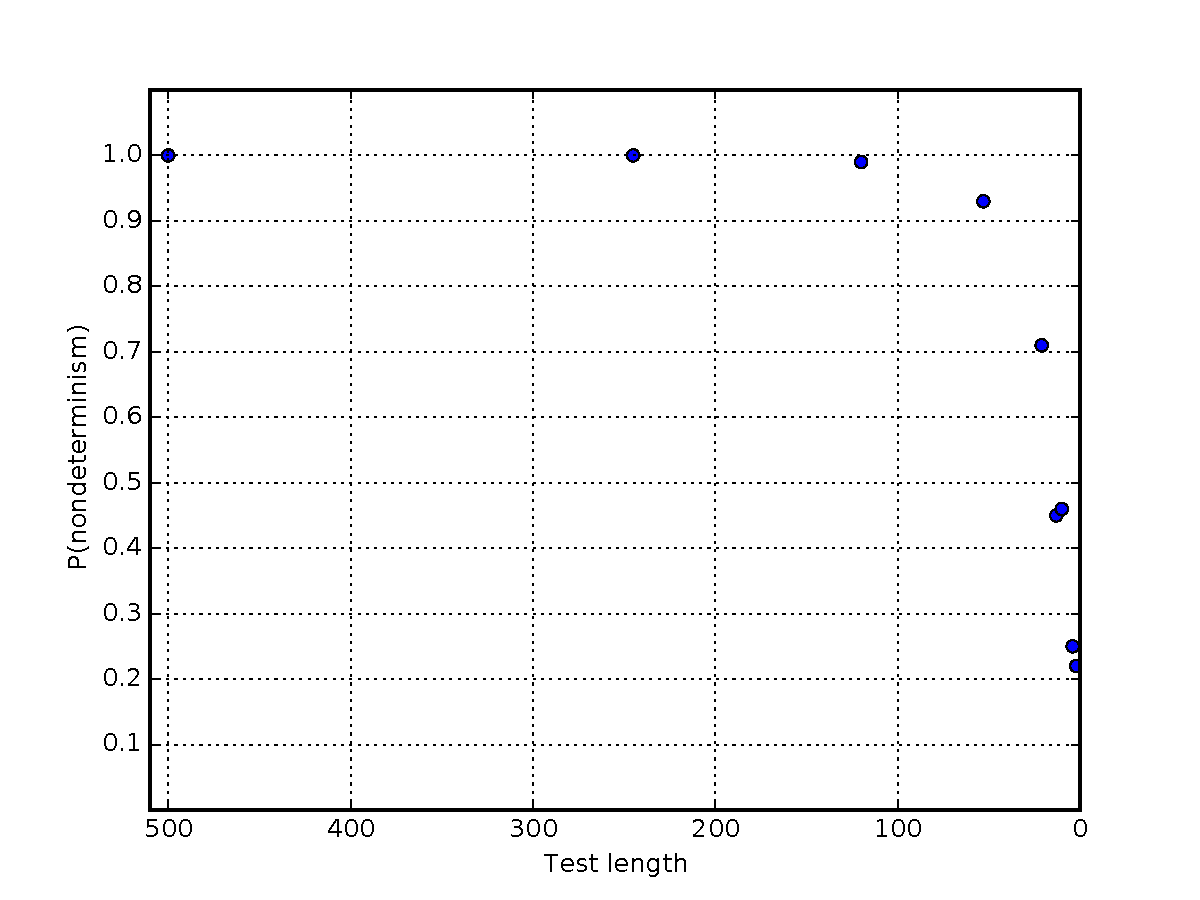
\includegraphics[width=\columnwidth]{lengthddmin}
\caption{No modification}
\label{fig:p1}
\end{subfigure}
\begin{subfigure}{0.30\columnwidth}
\centering
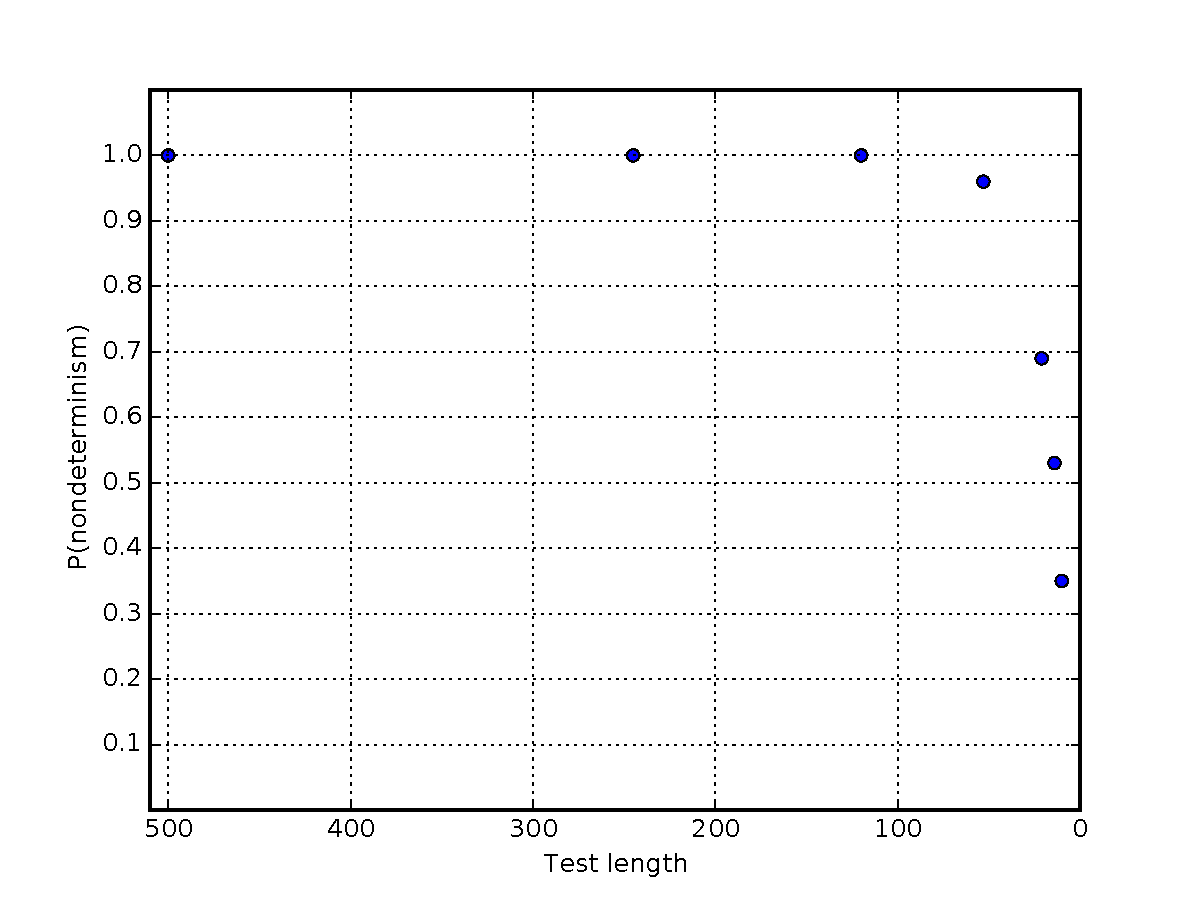
\includegraphics[width=\columnwidth]{lengthddminforcep}
\caption{N=100}
\label{fig:p2}
\end{subfigure}
\begin{subfigure}{0.30\columnwidth}
\centering
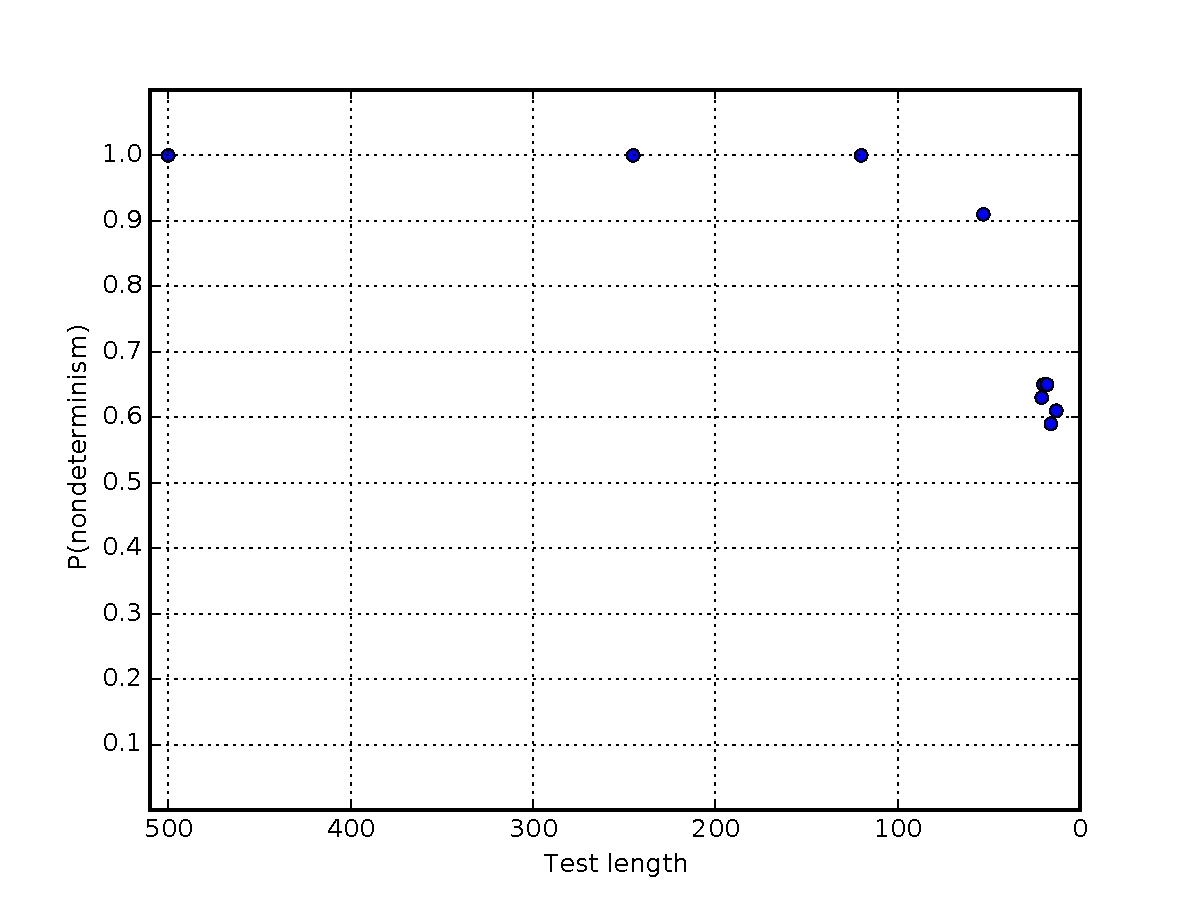
\includegraphics[width=\columnwidth]{lengthddminforceprep}
\caption{M=10, N=10}
\label{fig:p3}
\end{subfigure}
\caption{Reducing the same simple test; x-axis is time/changing
  $T_\mathit{CURR}$; y-axis is true $P(\mathit{PRED})$.}
\end{figure}

However, simply using delta-debugging off the shelf with a $\mathit{PRED}$
such as $P(\mathit{fail}) > 0.3 \wedge P(\mathit{fail}) < 0.7$, to force a test to be highly flaky, and force it to fail
sufficiently often to be used in debugging, will often produce
surprising and unfortunate results.  In many cases,
delta-debugging will indeed reduce the large test to a small subset.
And, in a technical sense, delta-debugging will work:  it will never
convert a nondeterministic test to a completely deterministic test,
because the reduced test $r$ that delta-debugging returns is always one
such that $\mathit{PRED}(r)$ has evaluated to true at least once.
However, if you run the resulting test, it will, in many cases, have a
$P(\mathit{fail})$ that is much, much smaller than
0.3, perhaps as low as 0.01.  In fact, we have often observed
delta-debugging taking a test that had such a high probability of
failure that we were unaware it was ``flaky'' (only hundreds of repeated executions showed there was
a small chance it could pass) and transforming it into a
test that only failed once in every 10 to 20 executions.
\emph{Delta-debugging can easily act as a flakiness multiplier.}  Why?

The problem is analogous to the problem of publication bias in
scientific fields \cite{ahmed2012assessment}.  We can think of each
application of $\mathit{PRED}$ to a candidate variant
$T_{\mathit{NEW}}$ as a scientific experiment.  A predicate like
$P(\mathit{fail}) > 0.3 \wedge P(\mathit{fail}) < 1.0$ cannot be evaluated by
determining the true probability of failure; we have no more direct access to
this value than a medical researcher has access to the true effect
size and direction of a proposed medical treatment; rather, the test must be
run some concrete number of times, and the number of failures counted.
Even if the number of samples $N$ is large, there is some
probability (based on the sample size) of a result that diverges
significantly from the actual probability of failure.  If the
predicate were run only once, and the number of samples reasonably
large, this would not matter.  However, test reduction algorithms explore a search
space that often contains thousands or millions of
tests.  The predicate is evaluated on each of these, and so
even with large $N$, it is likely that \emph{some} evaluation will
produce a poor estimate of $P(\mathit{fail})$.  At this point, reduction is
``stuck'' with the error, because the
algorithms usually do not allow backtracking.  After such a ``mistake,'' finding further
reductions will become harder, but may still be possible due to
another unlucky evaluation.  We define a \emph{false positive} in probabilistic
delta debugging as a case where $\mathit{PRED}$ evaluates to true, but
the actual probability constraints of $\mathit{PRED}$ are not
satsified (false negatives
also exist, but are less of a problem).

The analogy to publication bias is simple.  Assume that a paper in,
e.g., a medical journal will only be published if it shows that a
treatment is effective, with the statistical requirement that $p <
0.05$.  Even if no researchers are dishonest, 5 of every 100 papers published
in the journal will be report an effect with the wrong effect size or
even direction!  Now consider a ``hot'' topic, a kind of
treatment many research teams may investigate.  Major journals tend
not to publish papers that say ``this new treatment, which is not
established, may not work,'' (especially if the result is not ``we
accept the null hypothesis'' but only ``the experiment did not
show $p < 0.05$''), but they  are very likely to publish a paper
that says ``this exciting new treatment works!'' 
The \emph{bias} in
favor of positive results is shared by test reduction, which;
is much more influenced by cases where
$\mathit{PRED}$ holds than cases where it does not.
%The ``unpublished papers'' are invisible, magnifying the
%effect of the ``published'' experiments.

\begin{comment}
It is the combination of
a one-way bias on faulty evaluations (the consequences of a false
positive for the predicate are much greater than for a false negative)
and the huge number of experiments relative to error rate, that
produces bad results, akin to the magnification of effect sizes
in science due to publication bias.  The bias in delta-debugging tends
towards producing a reduced test where probabilities are much smaller
than demanded by a predicate, due to the pressure on delta-debugging
to produce shorter tests.  Shorter tests have smaller probabilities,
on average, due to two factors:  first, timing-induced nondeterminism
has a much smaller temporal space to operate in (the test may be over
before a ``time-bomb'' set by an operation goes off, for example), and second, if some
test operations introduce a small probability of nondeterminism, and
only many repetitions of those operations make the probability large,
small tests obviously, on average, have fewer instances of the
problematic operations.
\end{comment}

\subsection{Replication Mitigates  ``Publication Bias''}

In scientific literature, the most frequently proposed solution is the
use of replications:  repeated runs of ``successful'' experiments to
minimize the probability that a direction or effect size is a fluke.  One way to produce this effect would be to allow
reducers to backtrack if the probabilities observed in predicate
evaluations suddenly exhibit a strong discontinuity.  However, this requires
modifying the implementations, which is difficult and
sometimes not really feasible.  Ideally, the solution
should be implementable simply by modifying $\mathit{PRED}$ itself.

A costly but plausible solution is to make $N$ large in comparison to
the number of expected predicate evaluations performed during
delta-debugging.  However, given the large number of evaluations performed,
this will tend to make reduction extremely slow, since $N$ must be
very large indeed.  We propose
using a dynamic sampling approach, where $N$ is small, but if the
predicate evaluates to true, $M$ repeated true evaluations
(``replications'') are
required before the predicate is counted as holding.  To evaluate the predicate $\mathit{PRED}$ given $N$,
$M$, and desired probability bound $p$, the algorithm is:

{\scriptsize
\begin{code}
for $i = 0 \ldots M-1$
   $T =$ \# times $\mathit{PRED}$ is TRUE over $N$ evaluations.
   if $\frac{T}{N} < p$, return FALSE.
return TRUE
\end{code}
}

A set of $M$ repeated false positives with
$N = \frac{K}{M}$ samples each is much less likely than a false positive
with $K$ samples; so long as we accept the resulting bias in favor of
false negatives, we can therefore produce a reduced test with a
desired $P(\mathit{fail})$ much more cheaply:  the use of replications not only
means we only pay the full sampling price on rare occasions, but a
desired accuracy for $P$ can be obtained with a much smaller value $M
\times N$ than a non-dynamically-sampled $N$.  For example, if $\mathit{PRED}$
is $P(\mathit{fail}) \geq 0.5$, and the true probability for a candidate test
is 0.25, using $N=8$ will give a false positive rate of over 10\%.
Using 4 replications on just 2 samples ($M=4;N=2$) yields a false
positive rate of about 3.7\%, yet requires almost 60\% fewer
executions of the test.  The probability calculations for such comparisons are
relatively simple, but in real testing are
usually not very useful, since the true
probability distributions of test behaviors vary widely and
dynamically during the
delta-debugging process; gathering experimental data during a trial
delta-debugging run and tuning $N$ and $M$ to yield desired
results is  more effective.  In fact, by tuning $M$, any degree of confidence can be achieved, with
the basic tradeoff being between finding a test with the desired
probabilities, and the speed and effectiveness of reduction.
Because increasing $M$ makes false negatives more likely, larger $M$
will usually result in less-than-optimal reduction of the original
test.

To make the basic concepts, more clear, Figures
\ref{fig:p1}-\ref{fig:p3} graphically show the interplay of
delta-debugging and nondeterministic predicates for a simple example.
In the example, tests consist of a sequence of operations that behave
nondeterministically with (independent) probabilities of 0.01, 0.05,
and 0.10, respectively.  Figure \ref{fig:p1} shows one run of
delta-debugging on a test of length 500.  In
the course of reducing the test length to a test with only two
operations, the delta-debugging algorithm also reduces the probability
of nondeterminism from almost 100\% to about 20\%.  If we use a predicate that
``forces'' the test to behave nondeterministically at least half the
time, by sampling the predicate value 100 times and only returning
true when at least 50 of the evaluations report true, we see the
behavior in Figure \ref{fig:p2}:  the final test is slightly longer,
but still falls well short of our target of exhibiting nondeterminism
50\% of the time.  Finally, Figure \ref{fig:p3} shows what happens if
we use the same target of 50\% nondeterminism, but use only 10
samples, with 10 replications ($N$ = 10, $M$ = 10):  the test is not
much longer than in Figure \ref{fig:p2}, but the probability of
nondeterminism is above our target value, close to 60\% (and, as a bonus, many fewer
test executions are required on average for each check of the predicate).  